
We evaluate the performance of \Catra{} on~\NrBenchmarks{} instances of Parikh
automata intersection problems generated by the \OstrichPlus{} string constraint
solver~\cite{ostrich-plus} when solving the PyEx benchmarks, 
which are string constraints from symbolic execution that are known
to be hard for many solvers~\cite{pyex}. After generating an
initial~\InitialNrBenchmarks{}, we remove~\NrTrivial{} instances solved in under
five seconds by baseline as well as~\NrInvalid{} instances that were duplicates of other instances in the set.

 We also attempted to benchmark instances generated by
\OstrichPlus{} solving the Kaluza benchmarks~\cite{Saxena10:kaluza}
(\numprint{38227}~instances),
\iffalse
and pyex-len
(\numprint{791}~instances) benchmark suites\fi
but discarded them since they all turned out to be trivial for our tool
\Catra{}: every instance
could be solved in under five seconds, with a mean runtime of about 0.1s.
The benchmarks are run
on commit~\texttt{\commit} of \Catra{}\footnote{Github repository redacted for anonymity.}.

The benchmarks are executed in parallel across a cluster of identical
machines, \BenchmarkRig{}, as the sole job for each machine.  We compiled
the code using Scala~\ScalaVersion{} and executed the experiments
on~\JvmVersion{} with a maximum heap of~\MaxHeapSize{}. We used \Nuxmv{}
version~\NuxmvVersion{} invoked as a subprocess for each instance. Instances
were executed in batches of \BatchSize{}, each given a fresh JVM. Each JVM was
warmed up for \numprint{10}s on a random benchmark from the set before starting
to execute. We believe this represents a realistic use case where \Calculus{} is
used to support, e.g., a string solver. Experiments were executed in random order
for all backends. Each instance got a time budget of~\RuntimeTimeout{}.

All runtimes are measured in wall-clock time as observed by the JVM when
executing the instance, and exclude time spent parsing (usually far below
\numprint{0.1}s).

\subsection{Execution Time and Ability to Solve Instances}\label{sec:runtime}

\begin{figure}[t]
  \centering
  \begin{subfigure}[b]{0.49\textwidth}
    \includegraphics[width=\textwidth]{graphs/\commit-by-solver.pdf}
    \caption{The division of statuses per backend.}
    \label{fig:solve-division}
    \Description[A bar chart showing three bars, one per backend, illustrating how many instances they could solve]{The bars are divided by satisfiable and unsatisfiable instances. Baseline could seemingly only solve unsatisfiable instances, PC* could solve a few satisfiable and mostly unsatisfiable, and nuxmv could solve about twice as many unsatisfiable as satisfiable instances, and slightly less in total than PC*.}
  \end{subfigure}
  \hfill
  \begin{subfigure}[b]{0.49\textwidth}
    \includegraphics[width=\textwidth]{graphs/\commit-time-boxplot.pdf}
    \caption{The distribution of runtimes for solved instances per backend, assuming they were solved within the \numprint{30}s timeout.
    The whiskers use the default placement in Pandas, \numprint{1.5} times the IQR (interquartile range).}
    \label{fig:runtime-boxplot}
    \Description[A box plot showing the distribution of runtime over the three backends]{The middle box plot shows a tiny box centered around 0 seconds for the PC* backend, the rightmost box shows a bigger box between five seconds and 30 seconds for nuxmv, and the leftmost box shows a smaller box between 20 and 30 seconds for baseline. The whiskers of nuxmv span between 0 and the timeout, 60 seconds, while they are much tighter for PC*. On the other hand, PC* has a lot of outliers.}
  \end{subfigure}
  \vfill
  \begin{subfigure}[b]{\textwidth}
    \includegraphics[width=\textwidth]{graphs/\commit-cactus.pdf}
    \caption{The number of instances solved as the time budget increases, simulated from one \numprint{120}s-timeout run.}
    \label{fig:cactus}
    \Description[A cactus plot comparing the performance of nuxmv, PC* and baseline]{The line for baseline is strictly lower than the two others, and does not head upwards from zero until after 10 seconds of timeout, while the number of instances for nuxmv increases sharply until ca 10 seconds and then linearly after that. Lazy solves much more instances than nuxmv.}
  \end{subfigure}
  \caption{Evaluation of \Calculus{} solving Parikh automata problems generated by \Ostrich{}.}
\end{figure}


In \cref{fig:solve-division}, we show how many of the~\NrBenchmarks{} instances
the respective back-end could solve. A summary of their outcomes by instance
type is also available in \cref{tab:solve-status}. Note that many instances lack
a ground truth as they are solved by only one backend. We see that
\Calculus{} generally outperforms \Nuxmv{} on determining unsatisfiability, as
does baseline, while being similar at satisfiable instances. Both \Calculus{} and
\Nuxmv{} outperforms baseline on satisfiable instances. On satisfiable
instances, \Nuxmv{} and \Calculus{} have similar performance.

Baseline performs worse on satisfiable instances because it executes a heuristic
meant to detect unsatisfiability early, similar to~\cite{approximate-parikh}.
The heuristic is enabled since the improvement is significant compared to the
extra cost.

\begin{figure}[t]
  \centering
  \begin{subfigure}[b]{0.49\textwidth}
    \includegraphics[width=\textwidth]{graphs/\commit-duels-lazy-baseline-scatter.pdf}
    \caption{Per-instance runtime between baseline and \Calculus{}}
    \label{fig:duels:baseline}
    \Description[A scatter plot showing individual instances as dots compared to \Calculus{} and baseline]{The plot shows most dots at the bottom of the plot, with some plots collected at the right-hand side.}
  \end{subfigure}
  \hfill
  \begin{subfigure}[b]{0.49\textwidth}
    \includegraphics[width=\textwidth]{graphs/\commit-duels-lazy-nuxmv-scatter.pdf}
    \caption{Per-instance runtime between \Nuxmv{} and \Calculus{}}
    \label{fig:duels:nuxmv}
    \Description[A scatter plot showing individual instances as dots compared to \Calculus{} and \Nuxmv{}]{The plot shows flames of dots between the bottom and top, with a line of dots near the right-hand side corresponding to timeouts.}
  \end{subfigure}
\end{figure}


Finally, in \cref{fig:runtime-boxplot,fig:duels:baseline,fig:duels:nuxmv} and we compare
runtimes for solved instances between the backends. We see that \Nuxmv{} has a more even spread of runtimes up to \numprint{20}s,
while both \Calculus{} and baseline tend towards solving their
instances quickly or not at all, though \Calculus{} does have a long tail of outlier
instances that finish as the timeout increaseses.
Notably, \cref{fig:duels:baseline} shows that any instance solved by baseline in \numprint{30}s is also
solved by \Calculus{} in under \numprint{5}s.

\begin{table}
  \begin{center}
  \begin{tabular}{lrrr}
\toprule
backend & baseline & \Calculus & \Nuxmv \\
status after $30$s &  &  &  \\
\midrule
\textsc{Sat} & 6 & 3692 & 3288 \\
\textsc{Unsat} & 8958 & 15197 & 6356 \\
\bottomrule
\end{tabular}

  \end{center}
  \caption{Number of successful results within a timeout of \RuntimeTimeout{}.
  Instances solved by no backend within the timeout (about half of the set) are
  omitted from the table.}\label{tab:solve-status}
\end{table}

\subsubsection{Scalability}\label{sec:scaling}%
To investigate scaling we additionally execute \numprint{2000} randomly sampled
(without replacement) benchmarks with a \numprint{120}-second timeout. We add
runs of \Calculus{} with clause learning and restarts disabled, and with only
clause learning disabled to show the impact of \cref{sec:random-restarts}, and
\cref{sec:clause-learning} respectively.

A cactus plot showing the number of instances solved within a given timeout can
be seen in \cref{fig:cactus}. We see that \Calculus{} outperforms \Nuxmv{} in
general but that \Nuxmv{} might scale better on very long runtimes. This is
likely due to two factors. First, \Nuxmv{} is more mature than \Calculus{}, and
its more general model checking methods might pay off on more difficult
instances compared to problem-specific methods. Second, for longer-running
calculations clause learning as described in \cref{sec:clause-learning} might
matter more. As clause learning in \Catra{} is rudimentary and generalises
poorly across product computations, there is a performance hit.

\subsection{Evaluation in \Ostrich{}}\label{}%

\begin{table}
  \begin{center}
  \begin{tabular}{lrrrrrrr}
\toprule
solver & CA-Str & Competitors & \Ostrich{} 1.3 & \Ostrich{}+CA & Z3-Noodler & cvc5 & z3alpha \\
kind &  &  &  &  &  &  &  \\
\midrule
\textsc{Sat} & 6427 & 14207 & 9586 & 9930 & 7344 & 14069 & 13599 \\
\textsc{Unsat} & 5562 & 7574 & 7356 & 7387 & 5367 & 7377 & 7298 \\
\bottomrule
\end{tabular}

  \end{center}
  \caption{Number of solved benchmarks in the set of quantifier-free strings with
    linear integer arithmetic constraints (QF\_SLIA) at SMT-COMP~2023. The numbers are from
    the competition results, except for CA-Str, which is executed by us on the same 
    cluster as the competition with the same resources, and the two virtual portfolio solvers
    \Ostrich+CA and \textsc{Competition} which aggregate the best results from \Ostrich{}/CA-Str and 
    all the competition results for non-\Ostrich{} solvers respectively. }
  \label{tab:solve-status-smt-comp}
\end{table}

\begin{figure}[t]
  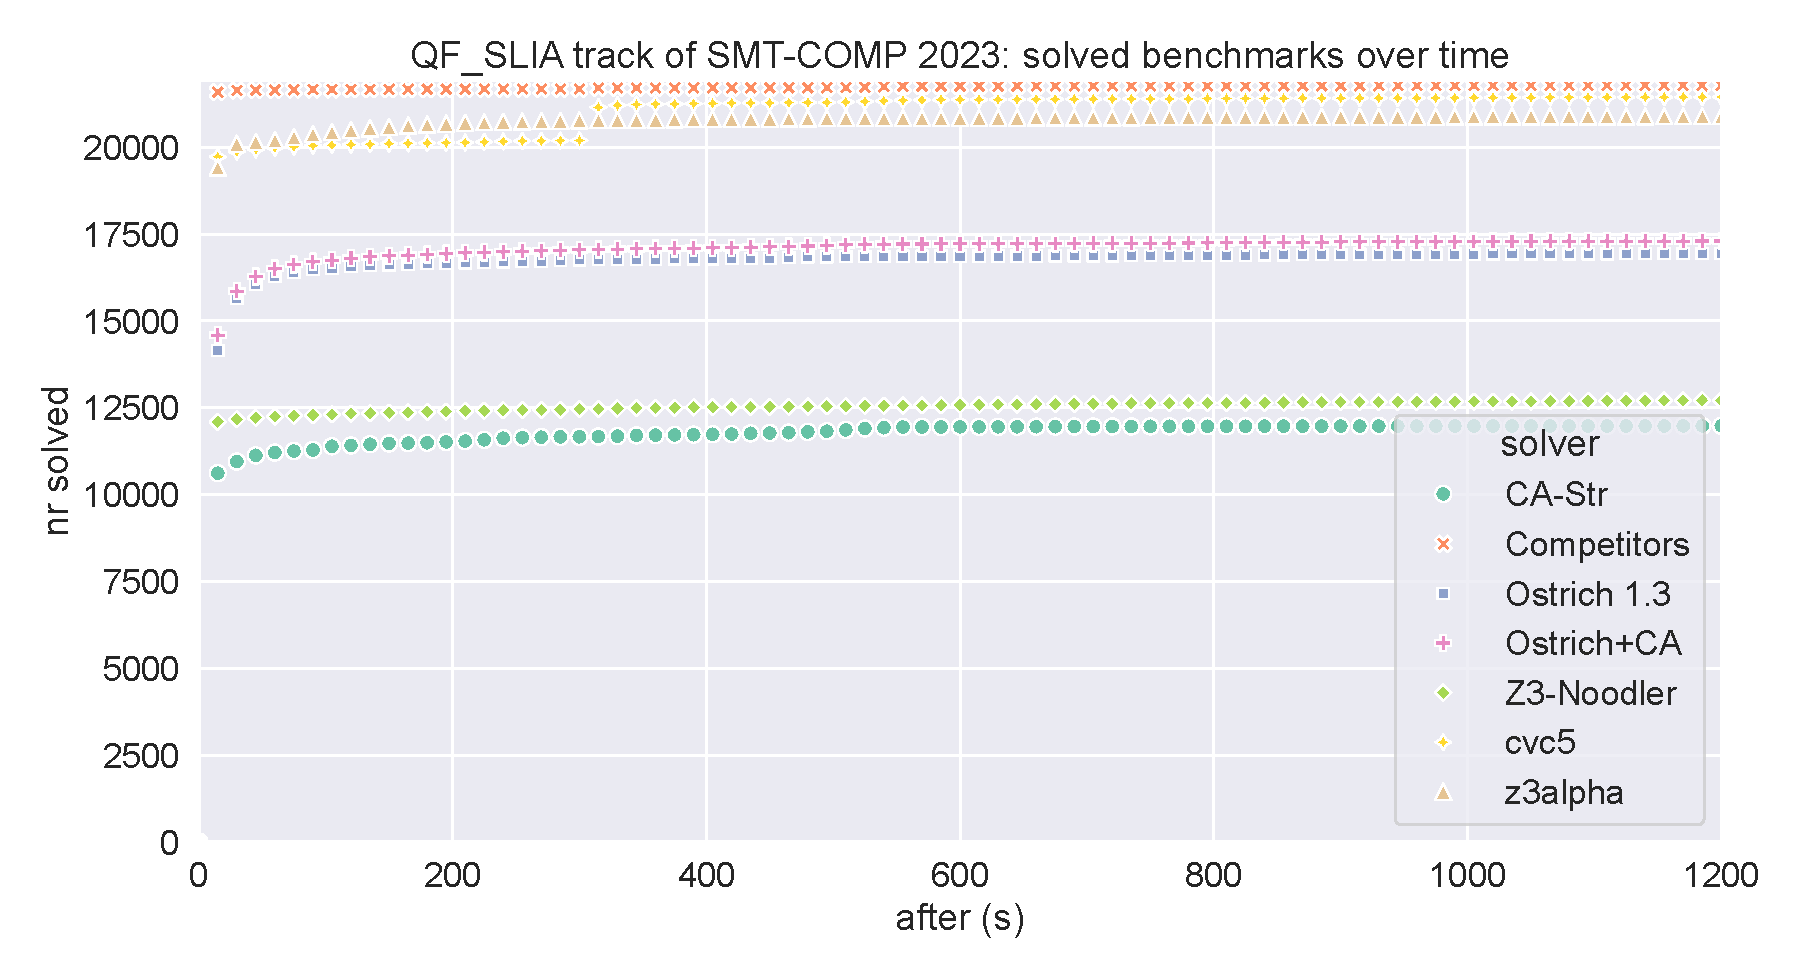
\includegraphics[width=\linewidth]{graphs/smt-comp-cactus}
  \caption{The number of instances solved in the QF\_SLIA track of SMT-COMP 2023
   as the time budget increases towards the competition limit of \numprint{20}~minutes.}
  \label{fig:smt-comp:cactus}
  \Description[A cactus plot comparing the performance of the solvers in the QF_SLIA track of SMT-COMP]%
  {The plot shows the results for the solvers Ostrich 1.3, CA-Str, Ostrich+CA, Z3-Noodler,
  cvc5 and z3alpha as number of solved instances (y-axis) after N seconds (x-axis). The
  topmost solver is the virtual portfolio "Competition", representing every non-Ostrich
  solver, followed by cvc5, after ca 200 seconds, after which it overtakes the previous leader, z3alpha.}
\end{figure}

To evaluate the effectiveness of \Calculus{} in a string solver, \Catra{} was
experimentally integrated as the Parikh automata product solver into the string
solver \Ostrich{}~version~1.3. \Ostrich{} is an independently developed solver
that participated in the recent
SMT-COMP~2023\footnote{\url{https://smt-comp.github.io/2023/participants/ostrich}},
winning the single-query track for quantifier-free strings (\texttt{QF\_S}), as
well as dominating other solvers on unsatisfiable string
benchmarks~\cite{smt-comp-23}.

 At SMT-COMP, \Ostrich{} competed using a portfolio of three different
 back-ends:
\begin{itemize}
\item \textbf{BW-Str:} a backward-propagation-based solver, not utilising
  Parikh automata~\cite{ostrich}.
\item \textbf{ADT-Str:} a solver based on algebraic data-types.
\item \textbf{CE-Str:} a re-implementation of the \OstrichPlus{}
  algorithm~\cite{ostrich-plus}, using Parikh automata and the
  encoding from~\cite{generate-parikh-image} (referred to in this paper as baseline).
\end{itemize}

For our experiments, we modify the CE-Str solver to apply \Catra{}
 (with \Calculus{} as its chosen backend)
instead of the previous baseline method, resulting in a new back-end
\textbf{CA-Str}. Combining the results from SMT-COMP for \Ostrich{}~1.3 
with our new results running CA-Str we construct a virtual 
portfolio~\Ostrich{}+CA that simulates running CA-Str as a fourth
back-end to \Ostrich{}. We similarly combine the results of all non-\Ostrich{} solvers
to obtain the virtual portfolio solver~\textbf{Competition}.

%As benchmarks, we again focused on the PyEx benchmarks~\cite{pyex}, of
%which we picked 1000~problems uniformly at random. We ran
%different combinations of the
%back-ends on those 1000~problems with a 120s timeout.
%
%The \texttt{QF\_S} track contains no Parikh automata intersection problems,
%however. For that, we need to look to the linear integer arithmetic
%(\texttt{QF\_SLIA}), where \Ostrich{} did worse in SMT-COMP. The evaluations in
%\cref{sec:scaling} use inputs generated by an older branch of CEFA-enriched
%\Ostrich{} on the PyEx benchmarks, which are part of the set used in the
%competition. In this section, we evaluated a version of \Ostrich{} using
%\Catra{} as its back-end \Fudge{on StarExec, the same cluster SMT-COMP ran on}
%on \numprint{1000}~randomly selected instances from the PyEx benchmarks. 
%
% comparison \Fudge{to the other provers of the 2023
%competition on the same benchmarks, as well as \Ostrich{} using the baseline
%back-end described in \cref{sec:implementing-baseline}}.

We extend the results of SMT-COMP~2023 with our modified \Ostrich{}
on the single-query string solving with linear integer arithmetic constraints
track (QF\_SLIA). We picked QF\_SLIA since
\Ostrich{} already performed well on the other two string solving tracks. In fact,
every solver, including \Ostrich{}, handled every benchmark in QF\_SNIA within the timeout.
Additionally, Parikh intersection problems would mainly be generated by \Ostrich{} when
solving constraints involving integers, meaning that CA-Str would be of little or no
help on the QF\_S track.

We obtain the results by executing \Ostrich{}~1.3 with CA-Str using
the same benchmarking infrastructure (the StarExec cluster)
and configuration that ran SMT-COMP~2023, combining our new results for CA-Str with the
published results of SMT-COMP~2023.
\footnote{StarExec Job ID 59410, \enquote{SMT-COMP 2023 single query final}, 
available at \url{https://www.starexec.org/starexec/secure/details/job.jsp?id=59410}.} 
Where avaiable, we use the revised, out-of
competition version of the results for solvers with bugs discovered during
the competition, including \Ostrich{} and Z3-Noodler. 
\footnote{StarExec Job ID 59668, \enquote{SMT-COMP 2023 single query final fixed} available at
\url{https://www.starexec.org/starexec/secure/details/job.jsp?id=59668}.}
Note that Z3-Noodler abstained on \numprint{70}~instances, and thus has a lower total number of results.
We used the parallel results for all solvers.

As can be seen from \cref{tab:solve-status-smt-comp} and \cref{fig:smt-comp:cactus},
integrating \Catra{} as a back-end
leads to gains both on satisfiable and unsatisfiable problems. On
satisfiable problems, the combination \Ostrich+CA is still
outperformed by cvc5 and z3alpha. On unsatisfiable benchmarks,
\Ostrich+CA now narrowly beats the other solvers squeezing past cvc5,
which is promising given that \Ostrich{}~1.3 (without CA-Str), cvc5, and z3alpha all show very strong
performance on this class of benchmarks.

These results are expected. It is known that automata-based string solvers (\Ostrich{}, Z3-Noodler) 
tend to perform better on unsatisfiable than on satisfiable benchmarks, compared to solvers
that do not utilize automata and directly work on regular expressions (cvc5, z3alpha).
This is not unexpected, as the computation of automata representations of regular 
constraints can be expensive, and might be unnecessary for satisfiable formulas.
In addition, the algorithm in \Ostrich{} has stronger theoretical completeness
guarantees than cvc5 and Z3-Str, and ensuring completeness often has an adverse
effect on performance in practice~\cite{ostrich,Z3-str,cvc5}.

The results show that \Calculus{} can be used to enhance the performance of an
automaton-based string solver. Moreover, the cactus plot in \cref{tab:solve-status-smt-comp} 
illustrates that
CA-Str is immediately useful, boosting the results for the \Ostrich{} portfolio
even at the first datapoint (though marginally). These results should be considered preliminary,
however, as we believe that a deeper integration of \Catra{} into string solvers
can lead to significant performance gains. In particular, the integration layer 
is currently too shallow to allow \Ostrich{} to learn clauses generated by \Catra{}
and additionally incurs overhead from serialising and deserialising the current Parikh
automata problem into \Catra{}'s input format.

\subsection{Threats to Validity}

The most obvious threat to validity would be an unsound implementation. To
address this we have validated all reported solutions made by \Calculus{} with
\Nuxmv{}. A previous version contained a race with random restarts during
product materialisation causing non-deterministic unsoundness in \numprint{0.7}
of instances. Additionally, both we and the artefact evaluation committee independently
discovered a soundness issue in CA-Str on one instance in QF\_S where the 
\texttt{QF\_S\slash{}20230329-automatark-lu\slash{}instance08425.smt2} instance was
incorrectly reported as \textsc{Unsat}. The underlying issue was that \Catra{} generated
a too broad blocking clause when encountering unsatisifiability stemming from 
an intermittent product accepting only the empty string during product materialisation. 
We implemented a fix for that bug and re-evaluated all benchmarks in SMT-COMP.

Since addressing those bugs we have observed no further soundness
issues in neither \Catra{} nor CA-Str. Benchmarking results for both runs are included
in the artefact of this paper, and show virtually identical performance characteristics.

The second threat to validity is our implementation of automata operations. As
\Calculus{} by design offloads some of the product computation work onto
\Princess{}, the baseline could be unfairly disadvantaged by a slow automata
product implementation. We believe this is not an issue since similar
performance issues with the baseline approach have been reported for other string
solvers, as well as for a previous implementation in \Ostrich{}. Additionally,
profiling shows that baseline spends most of its time in
\Princess{}, suggesting that the automaton implementation is not the bottleneck.
Finally, the difference in performance between \Calculus{} and baseline has been
robust under significant optimisation of the automata library, additionally
strengthening this thesis.

%%% Local Variables:
%%% mode: latex
%%% TeX-master: "main"
%%% End:
